\documentclass[a4paper]{article}
\usepackage[a4paper,left=2cm,right=2cm,top=1.8cm,bottom=2.8cm]{geometry}
\usepackage[english]{babel}
\usepackage{pictex,amsmath,amsfonts,amssymb,amsthm,verbatim}
\usepackage{fullpage}
\usepackage{fullpage}
\usepackage{fancyhdr}
\usepackage{algorithm,algorithmic}
\usepackage{multirow}
\usepackage{gensymb}
\usepackage{mathrsfs}

\setlength{\voffset}{-0.25in}
\setlength{\headsep}{+0.5in}
\setlength{\parskip}{1em}
\setlength{\parindent}{0em}

\def\vu{\mathbf{u}}
\def\vv{\mathbf{v}}
\def\vb{\mathbf{b}}
\def\vw{\mathbf{w}}
\def\vs{\mathbf{s}}

%Graphics packages:
\usepackage{graphicx, graphics}
\usepackage{tabularx, caption}
\usepackage{multirow, multicol}
\usepackage{setspace, tikz}
\usepackage{xcolor}
\usepackage{titlesec}
\usepackage{mdframed}
\usepackage{fancyhdr}
\usepackage{lastpage}
\usepackage[utf8]{vietnam}

\newmdenv[linecolor=blue,skipabove=\topsep,skipbelow=\topsep,leftmargin=5pt,rightmargin=-5pt,innerleftmargin=5pt,innerrightmargin=5pt]{mybox}

\newcommand{\quotes}[1]{``#1''}
\usepackage{minted}


%fancyhdr:
\setlength{\headheight}{40pt}
\pagestyle{fancy}
\fancyhead{} % clear all header fields
\fancyhead[L]{
 \begin{tabular}{rl}
    \begin{picture}(25, 15)(0, 0)
    \put(0, -8){
\includegraphics[width=8mm, height=8mm]{hcmut.png}}
   \end{picture}&
	\begin{tabular}{l}
		\textbf{\bf \ttfamily University of Technology, VNU-HCM}\\
		\textbf{\bf \ttfamily Faculty of Computer Science \& Engineering}
	\end{tabular} 	
 \end{tabular}
}

\fancyhead[R]{
    \begin{tabular}{l}
        \tiny \bf \\
        \tiny \bf
    \end{tabular}
}

\fancyfoot{} %clear all footer fields
\fancyfoot[L]{\scriptsize \ttfamily CC01 - Operating System (Spring 2019)}
\fancyfoot[R]{\scriptsize \ttfamily Page {\thepage}/ \pageref{LastPage}}
\renewcommand{\headrulewidth}{0.3pt}
\renewcommand{\footrulewidth}{0.3pt}

\begin{document}
    \begin{titlepage}
        \begin{center}
            HO CHI MINH CITY UNIVERSITY OF TECHNOLOGY, VNU HCM \\
            FACULTY OF COMPUTER SCIENCE AND ENGINEERING
        \end{center}

        \vspace{1cm}

        \begin{figure}[h!]
            \begin{center}
                
\includegraphics[width=3cm]{hcmut.png}
            \end{center}
        \end{figure}

        \vspace{1cm}

        \begin{center}
            \begin{tabular}{c}
                \multicolumn{1}{l}{\textbf{\LARGE OPERATING SYSTEM}} \\
                ~~\\
                \hline
                \\
                \multicolumn{1}{l}{\LARGE Lab 3: Process (Part 1/2)} \\
                \\
                \hline
                \\
                \hspace{5cm} Pham Minh Tuan - MSSV: 1752595
            \end{tabular}
        \end{center}
    \end{titlepage}

%Newpage:
\newpage

\section{\large Exercise: }
\subsection{\large Questions: }

\begin{enumerate}
    %1
    \item Describe the return values of fork() ?
    \begin{itemize}
        \item fork() returns a negative value if we cannot create a child process.
        \item fork() returns a zero value if the child process is successfully created.
        \item fork() returns a positive value, the process ID of the child process, to the parent process.
    \end{itemize}

    %2
    \item Run the example in Section 4 multiple times and observe the output of each time. Investigate the stability of the outputs and provide reasons as well as solutions for this phenomenon. (Your solution must ensure that the output must always be "Hello, World!") \\
    \paragraph{After running the above example multiple times, I receive 3 possible results occured:}
    \begin{itemize}
        \item The first result is shown at below:
        \bigbreak
        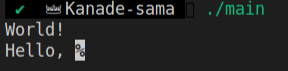
\includegraphics[scale = 0.5]{First_Result.png}
        \bigbreak

        \item The second result:
        \bigbreak
        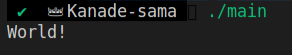
\includegraphics[scale = 0.5]{Second_Result.png}
        \bigbreak

        \item The third result:
        \bigbreak
        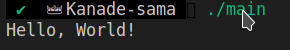
\includegraphics[scale = 0.5]{Third_Result.png}
        \bigbreak
    \end{itemize}

    \begin{itemize}
        \item The chance for the first and third result appear depends on how the Operating System (OP) first give the control to progress parents or child process.
        \item For the second result, since we the output of the program is shown in terminal which is line-buffered while the program run with full-buffered.
        \begin{itemize}
            \item When we call printf() to print the word into the console, it is not actually that we will immediately print it. The way printf() does is called buffering, printf() fill the word into the stdout initially.
            \item When the buffer is full, or when we print out new line ("\textbackslash n" character), it will be \textbf{flushed}. We can force the buffer to flush out immediately by calling \textit{fflush(stdout)}.
            \item In our program, after calling fork(), we have 2 process running concurrently, in my example the parent process is chosen to run first. However , after running \textit{printf("World!\textbackslash n)}, the "\textbackslash n" is observed and the output of terminal is line-buffered which means that the buffer will take the words in printf until it full or it reaches "\textbackslash n".
            \item In addition, we have 2 process running concurrently at the initial time, and every time we run the program in parent or child process especially child process since the printf() command does not have "\textbackslash n" character at the end so we do not know which line is stored in the buffer of the process, So sometimes we get the second result.
            \item In order to solve the second result, it has better to add "\textbackslash n" at the end of the printf() command so it will lead to only the first or third result.
            \item To ensure that the output will always be "Hello, World!", I suggest the \textbf{wait} command:
            \bigbreak
            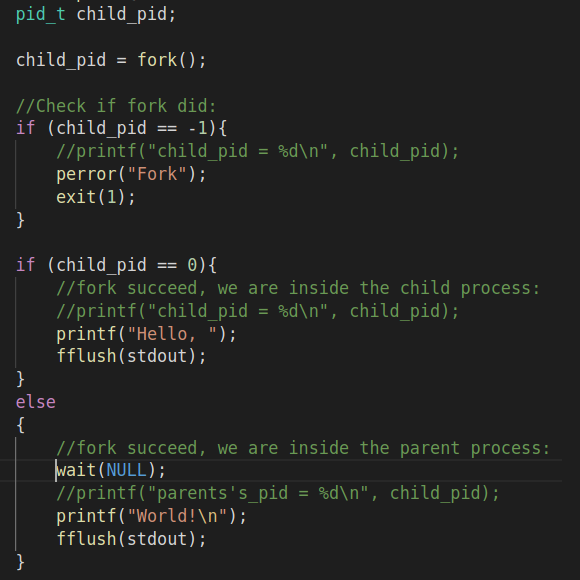
\includegraphics[scale = 0.5]{Solution.png}
            \bigbreak

            \begin{itemize}
                \item the \textit{wait(NULL)} command will wait for any child processes complete before running parents process.
            \end{itemize}
        \end{itemize} 
    \end{itemize}

    %3
    \item The result of LINE A is 5 because when we fork the program, there will be 2 processes at the time and the variable \textit{value} will have a independent value in both two processes, in child process it will be 20 and in parent process it will be 5.

    %4
    \item When a process creates a new process using the fork() operation, which of the following states is shared between the parent process and the child process?
    \textbf{Ans:} C. Shared memory segments
\end{enumerate}

\subsection{Programming Exercises}
\begin{enumerate}
    \item Problem 1: 
    \begin{itemize}
        \item Numbers.txt
        \bigbreak
        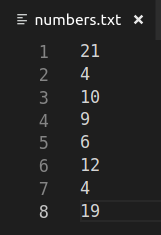
\includegraphics[scale = 0.5]{numbers.png}
        \bigbreak

        \item The result:
        \bigbreak
        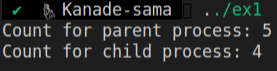
\includegraphics[scale = 0.5]{problem1.png}
        \bigbreak
    \end{itemize}

    \item Problem 2:
    \begin{itemize}
        \item The result:
        \bigbreak
        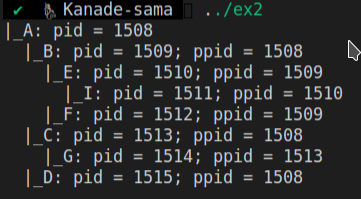
\includegraphics[scale = 0.5]{problem2.png}
        \bigbreak
    \end{itemize}
\end{enumerate}

\end{document}